\section{\asd Architecture}
\label{sec:arch}
In this section, we provide an overview of \asd architecture, and elaborate in more details on particular design decisions and challenges faced in its implementation. For the sake of clarity, in the rest of this discussion we will refer to the app that is being sandboxed by \asd as the \textit{managed app}. \\
\asd creates and runs the managed app within a dedicated container that enforces enterprise policies at runtime. 
\asd wraps each managed app in a sandbox that injects control hooks to intercept the app interaction with the external world. \asd offers two levels of interception both at Java and native code representations. Being able to intercept Java methods allows \asd to monitor and regulate all apps interactions via the Android API. However, apps might include C/C++ libraries (i.e., to boost performance). To monitor and possibly restrict the behaviour of these libraries, \asd also offers native code hooks. 
Our approach requires the installation of a single \stub for each managed app. The \stub is an app automatically generated by the app developer using the information contained in the manifest of the managed app. The \stub requests the same permissions as the managed app. The \stub contains only the shim code responsible for loading the managed apps at runtime and for dynamically retrieving enterprise-defined security policies. The \stub neither contains app code nor resources. For this reason, differently from repackaged apps, it can be submitted to the Google Play Store and installed on the devices as a regular app. Generating a \stub  is done using the \stubMaker provided by our framework and described in  Section \ref{sec:stubfactory}. However, it is important to understand that to generate a correct \stub, the manifest of the managed app has to be modified to set the values for the \shared and \proc attributes. Finally, the developer has to sign both the \stub and the managed app with the same certificate. \\

The use of the \proc and \shared attributes enables the creation of our sandbox. By using these two attributes, we are able to load the code of any app in the process space of the \stub. This approach has three main advantages: (i) \asd does not require to change any part of the code in the managed app and is able to work on stock Android without the need for root privileges and modifications to the Android OS; (ii) Our solution does not rely on the emulation of Android core services which could be cumbersome in terms of deployment and updating when a new version of Android is released; (iii) \asd does not need to re-implement several critical security checks normally performed by the Android system services which reduces the impact on performance. 

\iffalse
\begin{figure}[H]
\centering
\includegraphics[width=.5\textwidth, keepaspectratio, resolution=600]{lightboxmodel}
\caption{\asd enforcing managed apps}
\label{fig:lightmodel}
\end{figure}
\fi

%\begin{figure*}[htbp]
\begin{figure}[H]
%\subfigure[\asd high-level system design]{
\centering
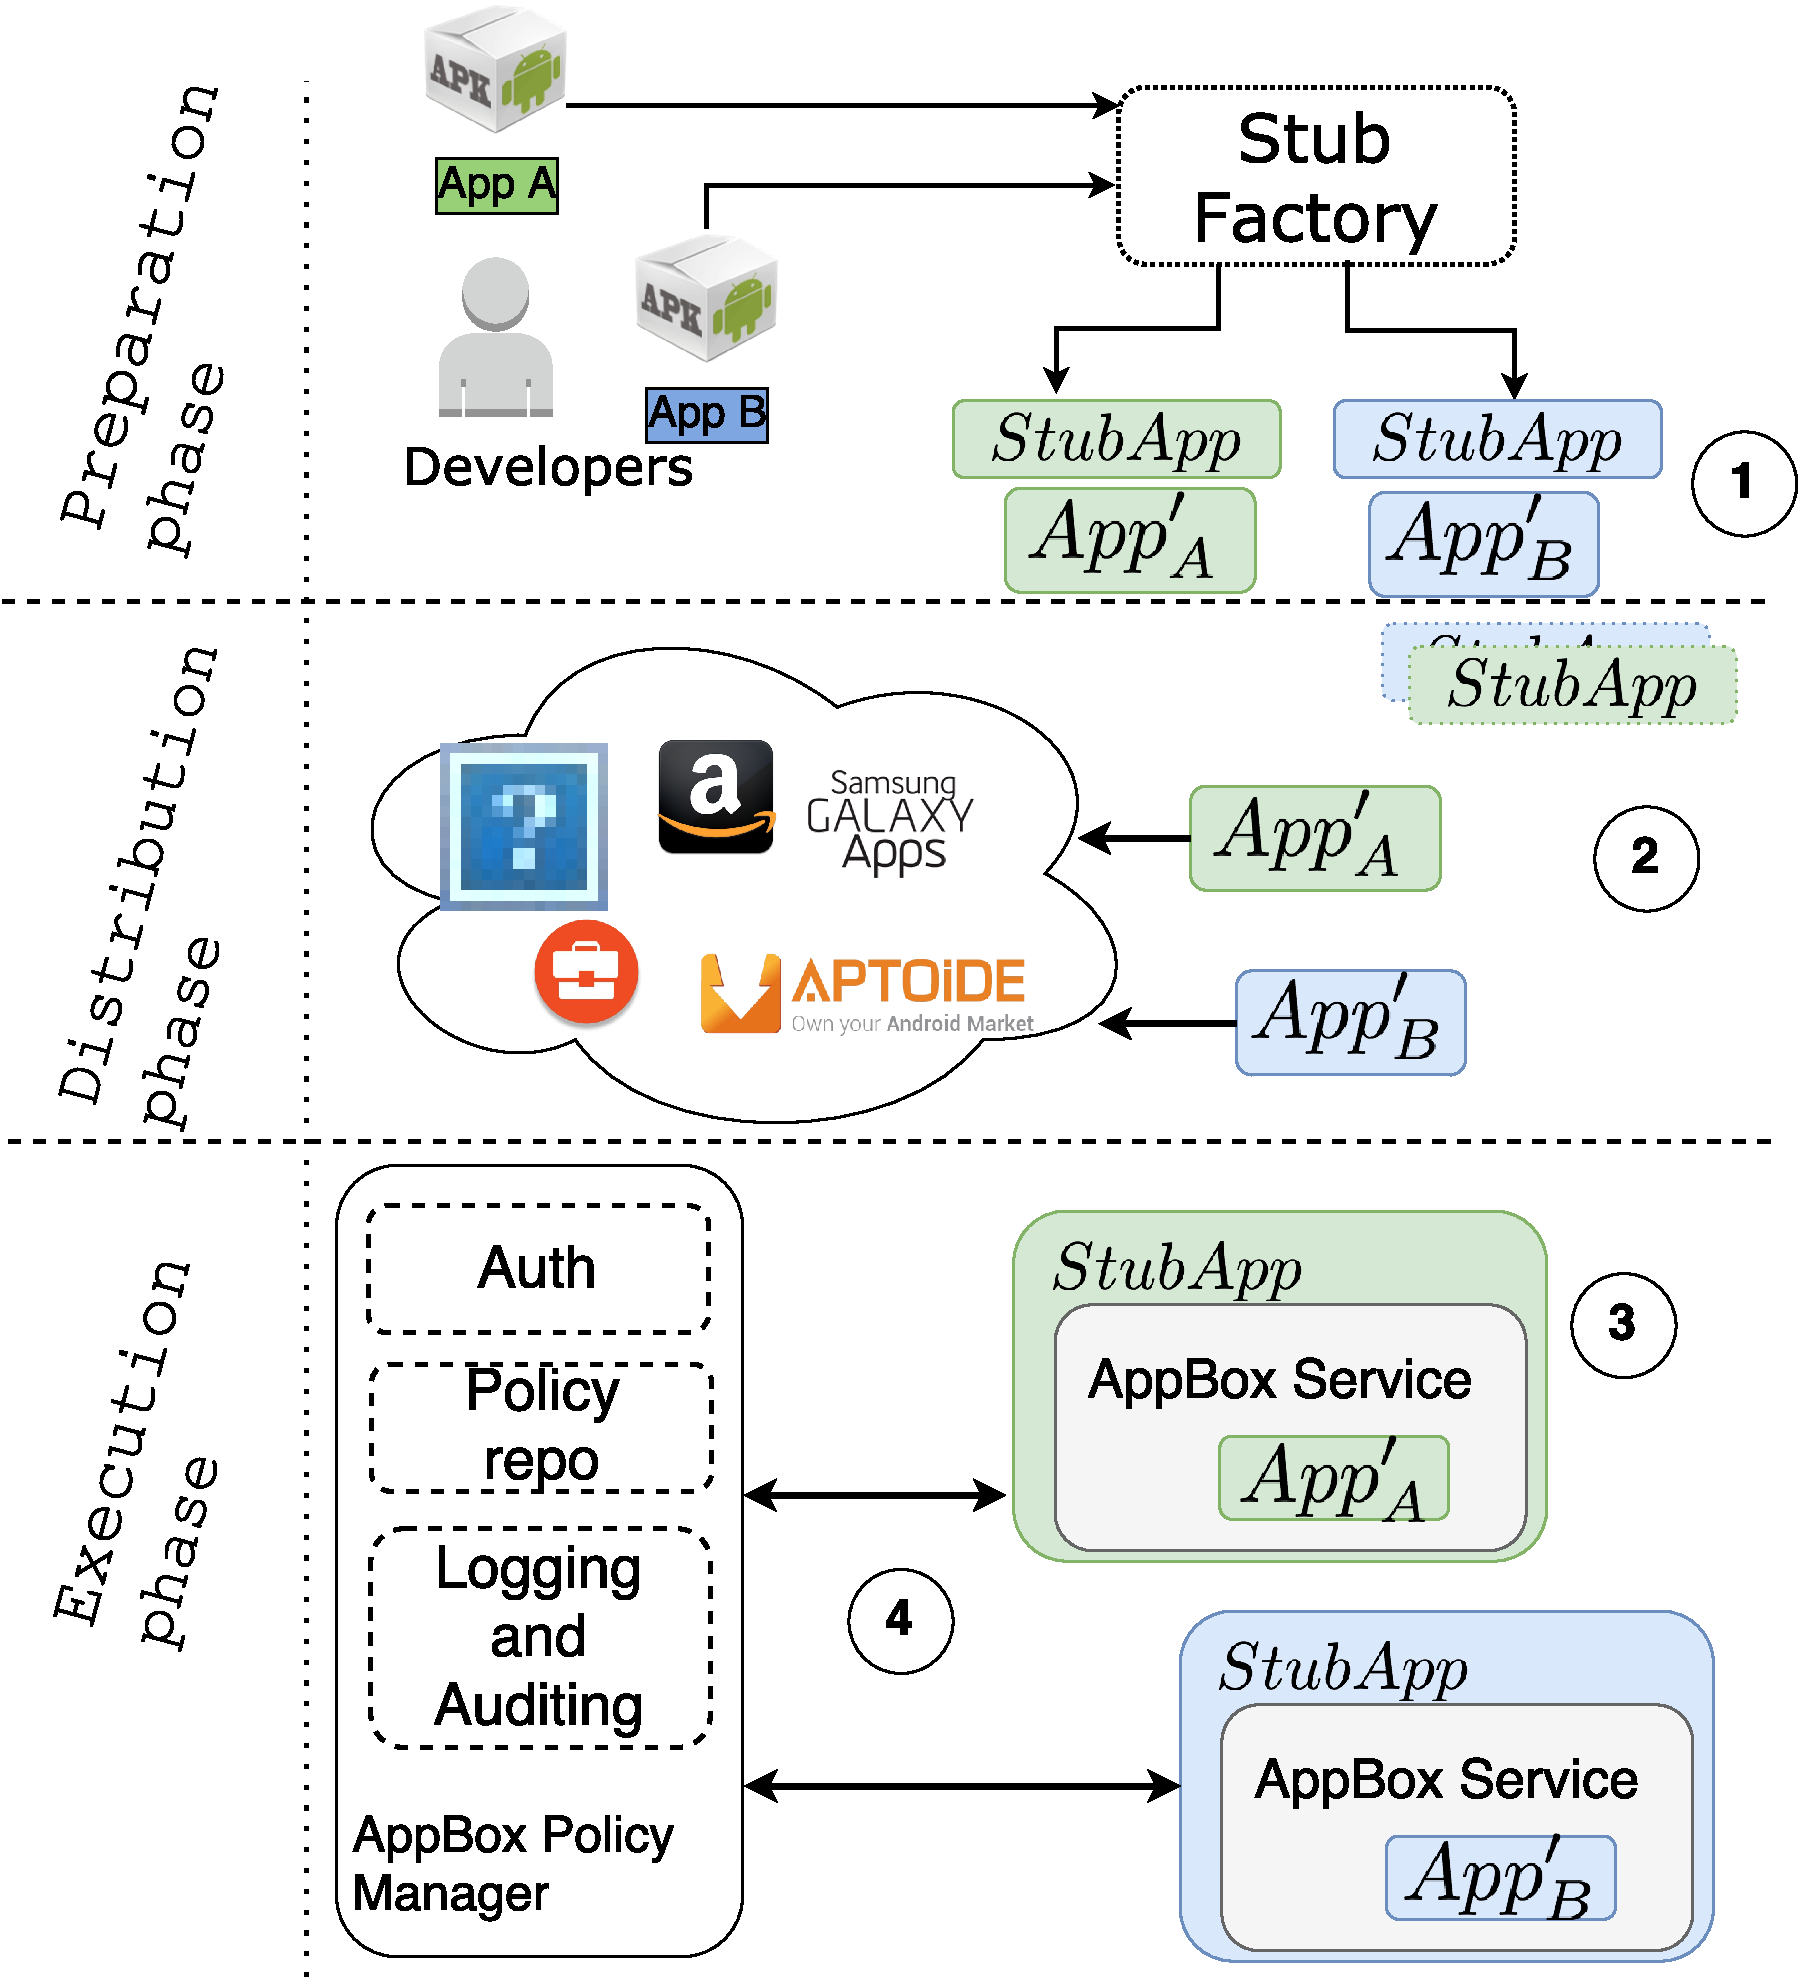
\includegraphics[width=.50\textwidth, keepaspectratio, resolution=600]{phases}
\caption{\asd design phases: Preparation , Distribution and Execution.}
\label{fig:sysdesign}
\end{figure}


\asd workflow consist of three main phases shown in Figure \ref{fig:sysdesign}: \textit{preparation}, \textit{distribution} and \textit{execution}.
During the preparation, the app developer creates the managed app ($App'$) and the \stub (step 1). Then, the developer distributes the managed app via any supported android market (step 2). During the distribution phase of the managed app the 
requested operations are exactly those which are actually followed by developers seeking to distribute their applications, no particular additional steps are required. Finally,  the user installs both  apps ($App'$ and the \stub) on the target device. During the execution phase, the \stub creates a sandbox to execute the managed app. The sandbox is responsible for monitoring the managed app's behaviour and enforce the policies (step 3), specified by the enterprise, offered via \asd Policy Manager instance (step 4). 

In the following, we provide a description of the components involved in each phase.

\subsection{Preparation phase} \label{sec:stubfactory}
To be able to manage an app with \asd, the developer has to create the \stub and a managed app, as shown in Figure \ref{fig:sysdesign}. This steps is performed by the developer using the \stubMaker, a set of python scripts along with a small DEX file containing the actual stub code.   
Another interesting aspect is that because the \stubMaker only operates at the level of the manifest file, the managed app and \stub can be created even if the original app code is obfuscated. 
It is worth noting that none of the existing approaches for app behaviour customisation on stock Android devices, are able to deal with obfuscated apps. 

In the following, we assume that $App$  is an app behaviour that an enterprise wants to customise using \asd. Using the \stubMaker, the developer generates the managed app, indicated as $App'$, and the stub app, indicated as $StubApp$. Finally, both the \stub and the managed app $App'$  must be digitally signed by the developer. 

\begin{figure}[H]
\centering
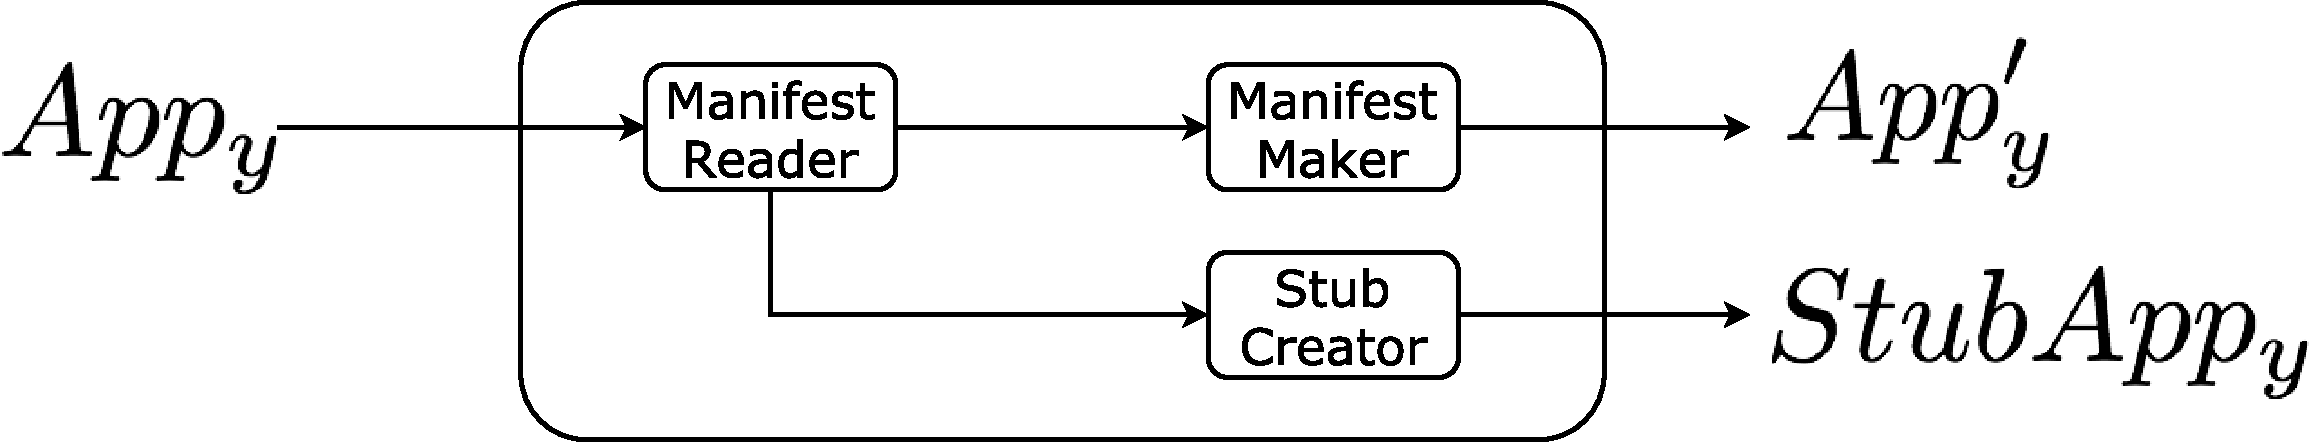
\includegraphics[width=.45\textwidth, keepaspectratio, resolution=600]{stubbo}
\caption{StubFactory and its components}
\label{fig:stubfact}
\end{figure}

As shown in Figure \ref{fig:stubfact}, the \stubMaker first extracts and decodes the Android manifest from $App$ (obtained as APK file) using the \textbf{Manifest Reader}. This component parses the input app's manifest collecting information such as  package name, main activity as well as requested permissions. Furthermore, it checks if the manifest contains components of $App$ defined to run across multiple processes. If this is the case, then the names of these components are added to the manifest of the \stub such that any additional process created by the app will be monitored by a dedicated sandbox instance. It is worth noting that the Android manifest is always in cleartext even in the case of heavily obfuscated apps. \\

Next, the \textbf{Manifest Maker} creates a new  manifest for $App'$ to include both the attributes \shared and \proc. If $App$'s manifest contains the broadcast receiver for the boot completed intent, then this will be removed from the $App'$'s manifest. This is to prevent the situation in which $App'$ might be launched before \stub. 

The last step is to create $StubApp$ through the \textbf{Stub Creator}. This last component first creates the manifest for the $StubApp$ with info previously collected by the Manifest Reader. The  $StubApp$'s manifest will have the same permissions as $App$. By default, $StubApp$'s manifest will have the broadcast receiver component for the BOOT\_COMPLETED system message. In this way, all the \stub installed in a device will start as soon as the booting phase is completed. If the $App$'s manifest also contained this broadcast receiver, then the $StubApp$ will act as a proxy and forward the boot completed intent to $App'$. \\

It is worth noting that $App$ and $App'$ have exactly the same  bytecode. In fact, the \stubMaker only operates on the $App$'s manifest to output \stub and  $App'$.  
The developer is able to create as many \stub as she may need to satisfy customers' requests. In fact, to iterate the preparation steps the developer is asked to create a new certificate, which will be offered to each customer.

Application updates are distributed via the application market as an usual APK file, the developer needs to sign them by the same certificated used at the first place. From the developer point of view, it looks exactly the same when it comes to publish managed app updates. In fact, there is no need to manually propagate those updates to each managed app code. The only step asked to the developer is to create a new managed app by means of \stubMaker components, as discussed before, thus updating an application is trivial as creating a managed one derived from the original application. In most cases there is no need to create a \stub again, this operation is requested only if the app's manifest file has been modified by that update.

In the following, we  discuss the details of the distribution phase.

\subsection{Distribution phase}
Once a developer has built an application she is interested in distributing its product to seeking consumers.  
In this phase the developer distributes applications as usual via any supported market.

There is no specific limit on apps distribution imposed by \asd, in any case who owns the \stub is able to control the associated managed app ($App'$).

\asd does not require any additional user interaction to complete an application update via the employed market and the developer does not need to accomplish any particular operation in order to distributed updates of managed apps. Whenever a new update is developed, in order to distribute it the developer uses the \stubMaker to automatically produce an updated managed app version (same operations done by preparation phase). Thanks to our approach the developer does not need to redistribute the \stub component. 

\subsection{Execution phase}
After the preparation step, both $StubApp$ and $App'$ are deployed on a device running stock Android OS.

The execution of the managed app is done by the \textit{\asd Service}. The \asd Service is a process created by the \stub that loads and executes the code of the managed app $App'$. Because the \stub and the \asd Service share the same process space, it is possible to inject hooks at runtime into managed app's virtual memory (which runs inside the \asd Service). These are the hooks that enforce the desired policy. By sharing the same UID through the use of the \shared attribute, the \asd Service is able to access all the private files of the managed app. In \asd, the managed app is dynamically instrumented by means of functions interposition on both Java and native levels, this enables the enforcement of security policies related to Java APIs and native code. The \asd Service modifies the memory of the managed app to inject hooks capable of intercepting calls to Java methods and to syscalls. The  mechanism is transparent to the managed app and new versions of the target app can be easily managed without the need to change either the \stub or the \asd Service. \\

The biggest technical challenge at this point is to guarantee that the managed app execution will be entirely confined within our sandbox. Android  offers a considerable number of features for apps to communicate with each other and share functionality. These features are accessed through callbacks such as broadcast messages, intents, and IPC. Care must be taken to avoid that these mechanisms can be exploited to let the managed app to execute outside its  sandbox.

In particular,  the exported components of an app, include the main activity that is always exported by default, can receive explicit intents sent by any app. When this happens, usually Android starts the exported component into  a new process. If not handled properly, this could be an issue because effectively could result in a managed app starting in a process outside its sandbox. However, before starting a new process, Android searches if there is already a process where (1) the process name matches the requested component's name; (2)  the process UID is the same as the one assigned to the app in which the target component has been defined. Thanks to the combination of both attributes \shared and \proc the \asd Service is sharing the same process name and UID, hence any intents sent to any exported component of a managed app will be captured and executed within the \asd Service.    


\subsubsection{\asd Policy Manager}
\label{sec:polman}
\asd Policy Manager is console application deployed on the enterprise infrastructure intended to be used by IT administrators. Through the \asd Policy Manager an administration can define new policies and deploy them on the enrolled devices. Once the managed application has been started, the \asd instance manages the authentication process with the Policy Manager. 

It is worth noting that new policies can be dynamically distributed as soon as the enterprise IT department loads them into the policy repository. Furthermore, \asd supports logging and auditing features  that can be configured for each managed app, in order to monitor the status of the app while running.

\subsubsection{\stub and \asd Service} \label{sec:stub}
The \stub is the key component for the realization of the \asd Service. The \stub is responsible for creating the sandbox process where the managed app will be executed as shown in Figure \ref{fig:stubapp}. When a managed app is launched, first the \stub creates the  \asd Service in a separate process (step 1) and invoke the \textit{prepare} method via the Binder to set up the interceptors (step 2). Then, the \stub retrieves the set of policies and the hooking library (step 3) specific to the managed app from the \textit{\asd Policy Manager}. The \asd Service loads the hooking library to  instrument its virtual memory. Once the instrumentation is completed, managed app's code will be loaded by directly invoking the \textit{bindApplication} method exposed by the \textit{ApplicationThread} class. As a result, managed app is loaded and its main activity is executed within the \asd Service (step 4). 


\begin{figure*}
\centering
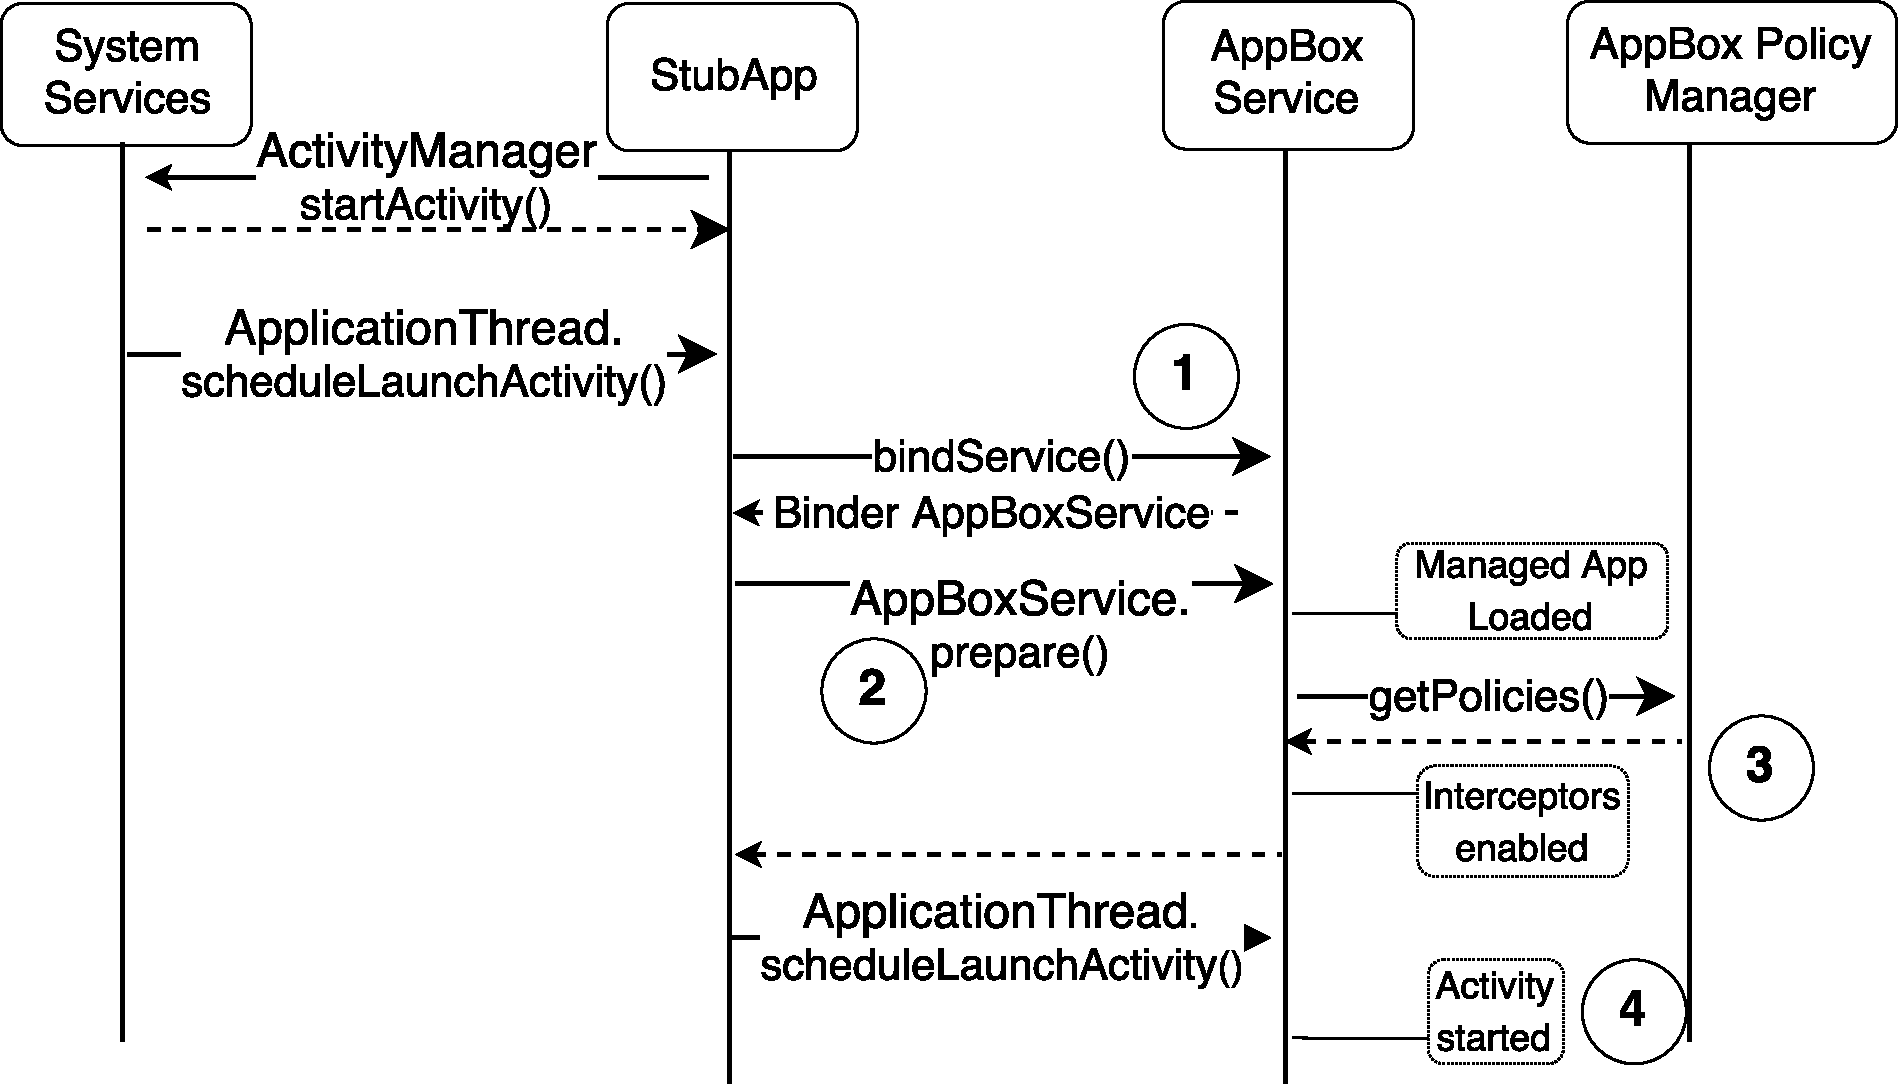
\includegraphics[width=.8\textwidth, keepaspectratio, resolution=800]{lbservice}
\caption{\asd enforcing managed apps}
\label{fig:stubapp}
\end{figure*}

As soon as the library is loaded, its virtual memory is altered to achieve functions interposition by means of different techniques, as detailed in Section \ref{sec:hook}. 

Before the managed app can be executed, the \stub has to create the right Android context for that app. This operation is performed by calling the Android API method \textit{createPackageContext}\footnote{\url{https://developer.android.com/reference/android/content/Context.html\#createPackageContext(java.lang.String, int)}} specifying  the CONTEXT\_INCLUDE\_CODE flag. 
As an entrypoint, the \stub declares in its manifest an \textit{Application}\footnote{\url{https://developer.android.com/reference/android/app/Application.html}} class, that is the first app component loaded by Android before any other app code. 
%In this way, we can make sure that the \asd sandbox is created before the execution of the managed app starts. 
If the managed app has components that need to be executed in different processes then the \stub will start several \asd Services, one for each component of the app. 


\subsubsection{Java and Native Interceptors} \label{sec:hook}
The Java interceptors in \asd are an extended versions of the ArtDroid  hooking framework \cite{costamagna2016artdroid}. However, compared to ArtDroid, \asd Java interceptors are able to hook static Java methods by implementing the approach proposed in \cite{wissfeldcallee}. 
The Java interceptors can operate at the level of Java methods defined within the managed app. We are able to intercept all calls to monitored Java methods including either calls via Java reflection, native code or dynamically loaded code. The intercepted calls are redirected to the specific Policy Enforcement Point (PEP) where the actual user-defined policy is enforced. Java interceptors achieve transparent hooking by means of memory instrumentation. It  fully supports both the DVM and ART Android runtime. The interposition offered by the Java interceptors permits to monitor the access an app performs to  Android APIs to interact with system services (i.e., LocationManager, TelephonyManager) and the Android environment (i.e., Context, SharedPreferences). In Android, apps can also  invoke these APIs from native code via the JNI interface. In addition, in Android native code is allowed to perform direct Binder transactions without invoking any Android Java method. To address this, \asd relies on the Native interceptor to intercept these calls that could bypass the policies defined at the Java level.

\asd offers also  native functions interposition by means of \textit{inline hooking}, a well-known technique~\cite{inlinehook} that basically permits to redirect a function call to another function under the control of a monitor process. In contrast with the GOT patching techniques, \asd can intercept calls to  any native function not only the ones to  global symbols (i.e., calls to functions defined in the same module will not generate entries in GOT). \asd allows to intercept calls to functions like \textit{open, connect, read}, access to the Binder via the \textit{ioctl}, etc. In this way we can  monitor if the managed app tries to access system services directly via native call to the \textit{ioctl} function. Enabling native interceptors is optional. For instance, if an app does not use its own native libraries then native interceptors can be disabled. However, if the managed app dynamically loads a native library then \asd can automatically enable the native interceptors layer.
         

%///////////////////
\iffalse
\begin{figure*}[htbp]
\centering
 % Store largest image in a box
  \savebox{\imagebox{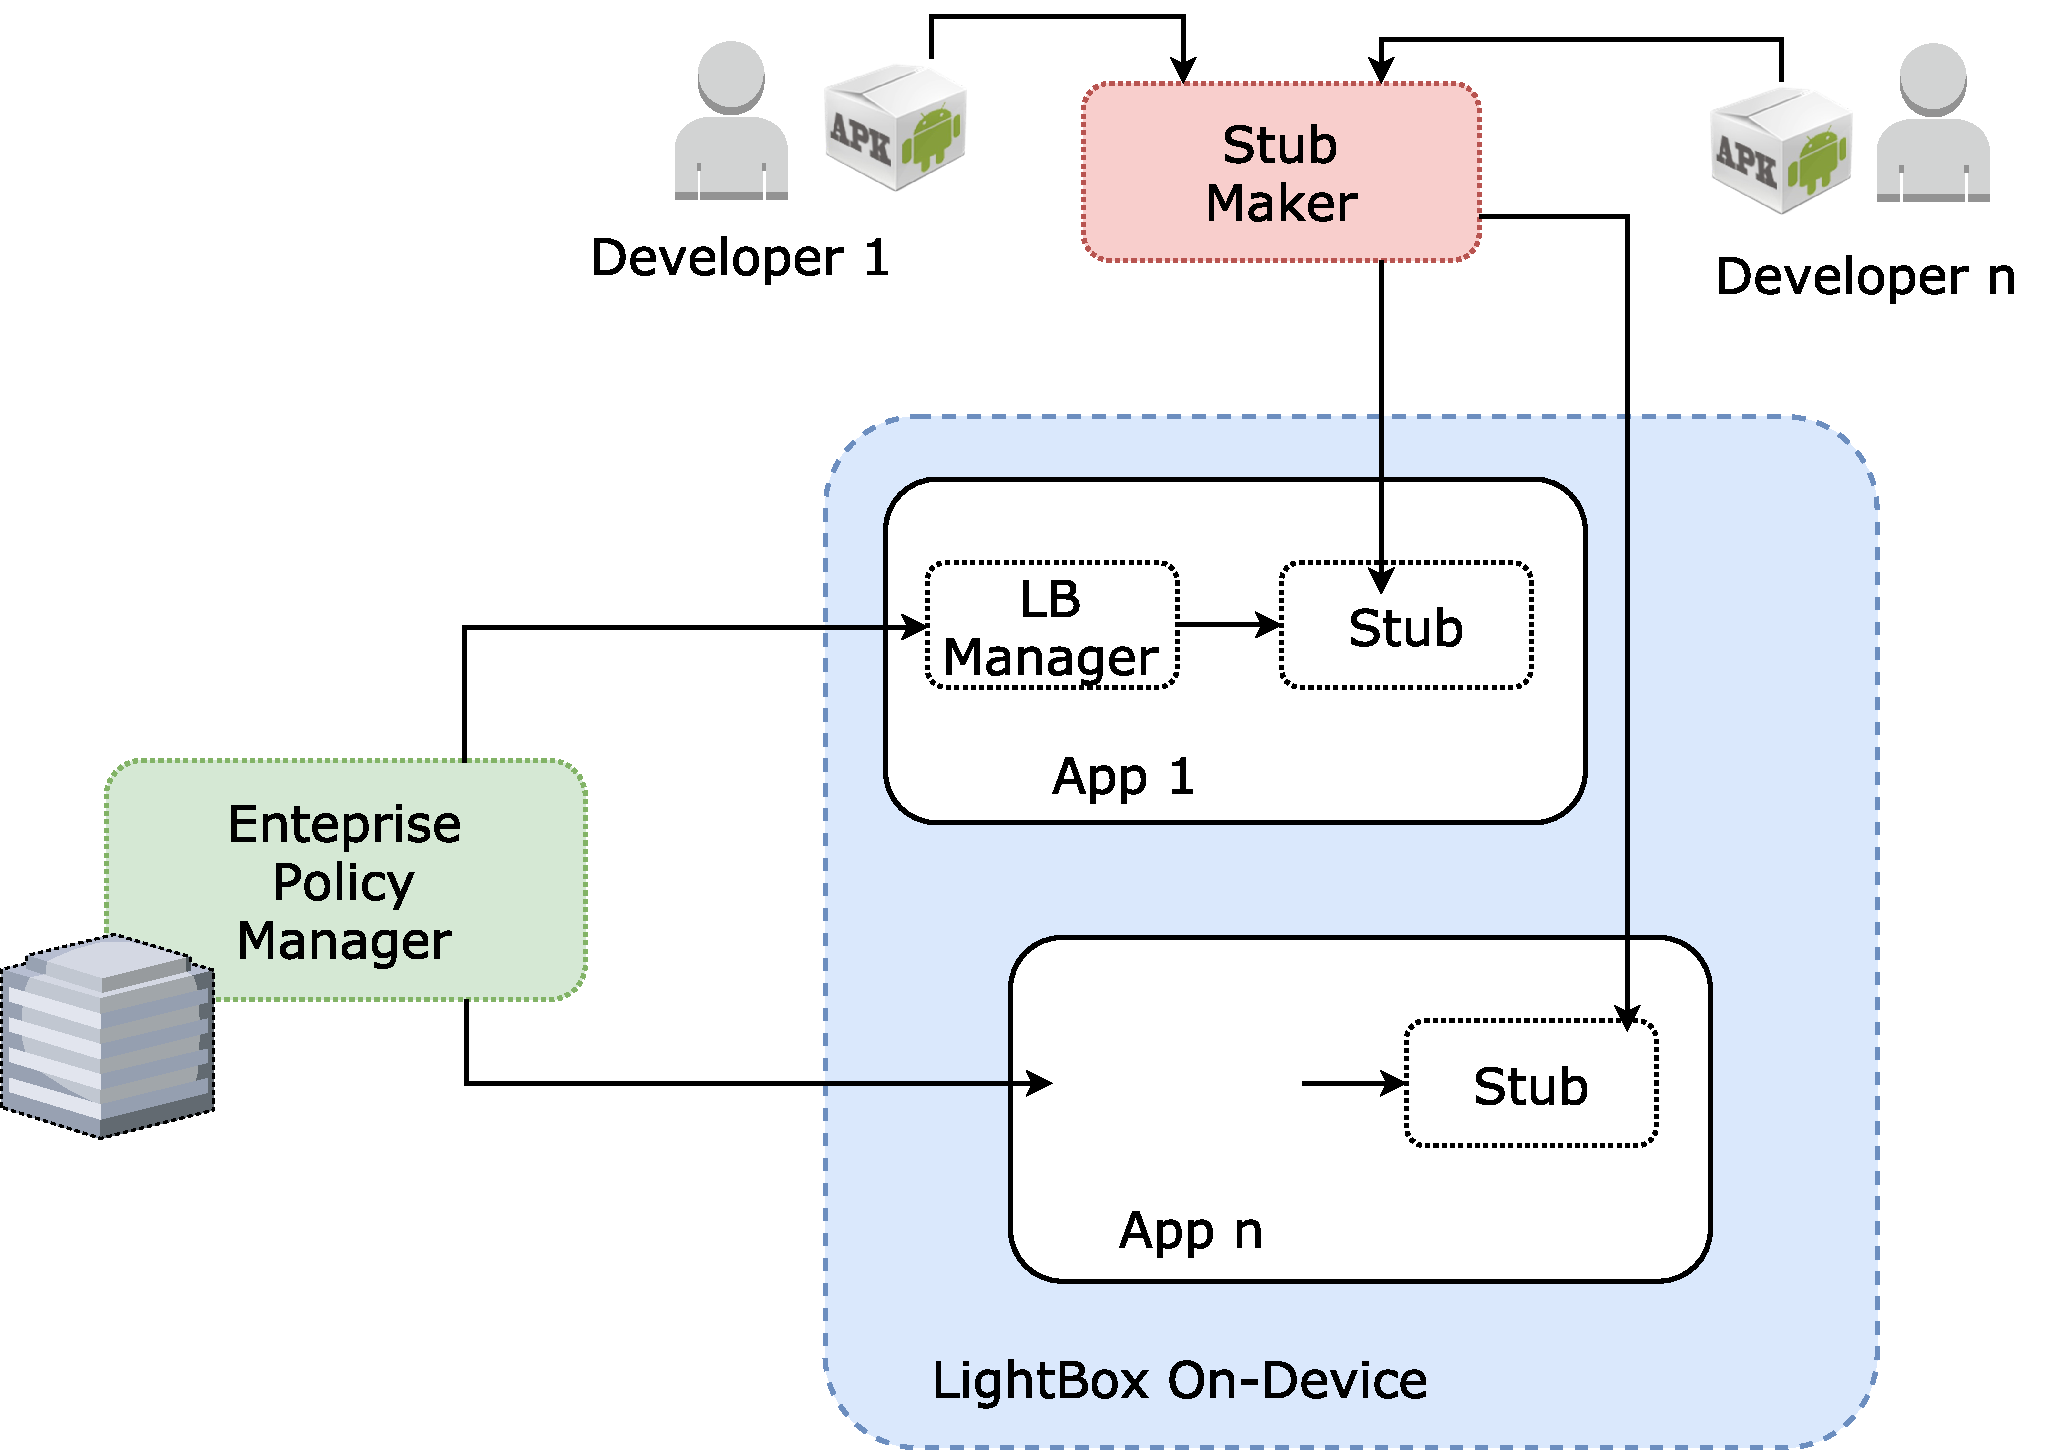
\includegraphics[width=.4\linewidth,height=150pt]{design_overview}}%
  \begin{subfigure}[]{}
    \centering\usebox{\imagebox}% Place largest image
    %\caption{LightBox high level design}
  \end{subfigure}\qquad
  %Nothing
  \begin{subfigure}[]{}
    \centering\raisebox{\dimexpr.5\ht\imagebox-.5\height}{% Raise smaller image into place
      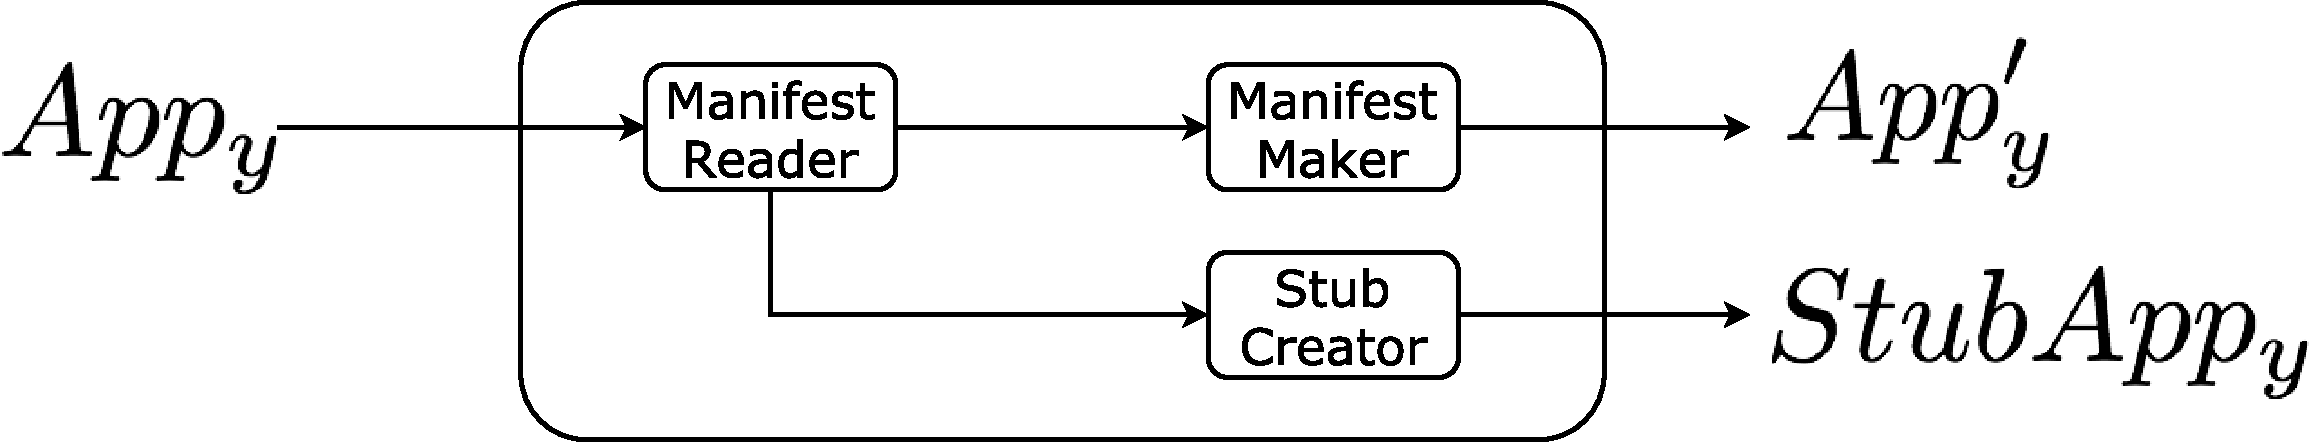
\includegraphics[width=.5\linewidth,height=5pc]{stubbo}}%
    %\caption{StubFactory}
  \end{subfigure}
\caption{\asd (a) system design creation, (b) \stubMaker }
\label{fig:lightbox}
\end{figure*}
\fi
%//////////////////////////////
\iffalse
\begin{figure*}
	\centering
	%\subcapraggedrighttrue
		\begin{tabular}{@{}c@{}}
			\subfigure[a]{
				\centering
            	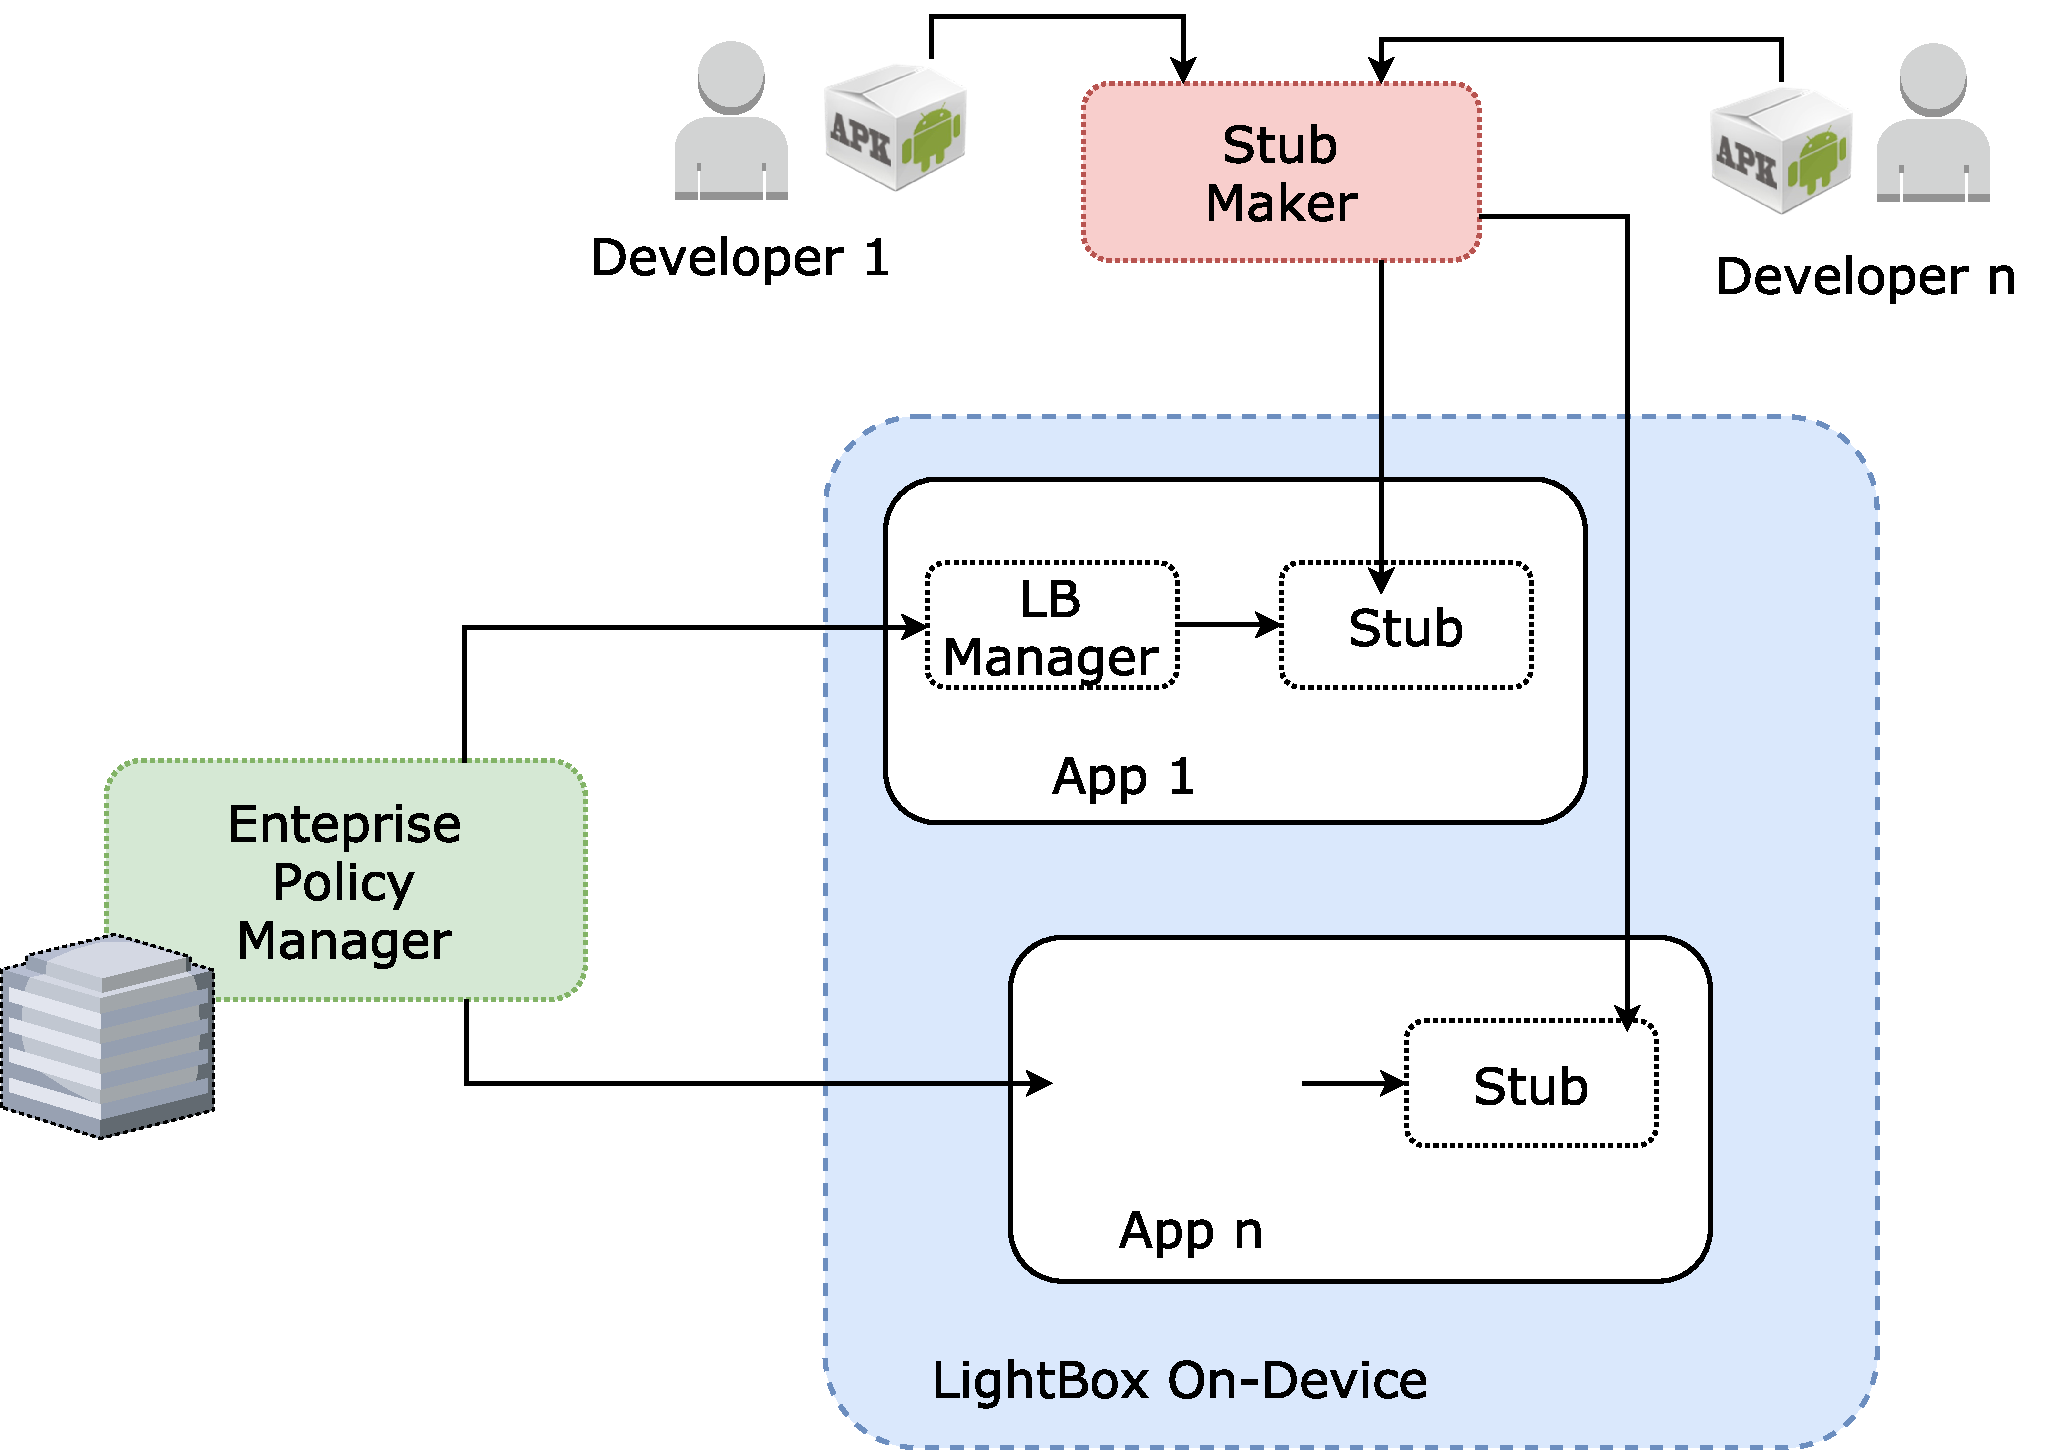
\includegraphics[width=5cm]{design_overview}}
				
		\end{tabular}
		\begin{tabular}{@{}c@{}}
			\subfigure[b]{
            	\centering
                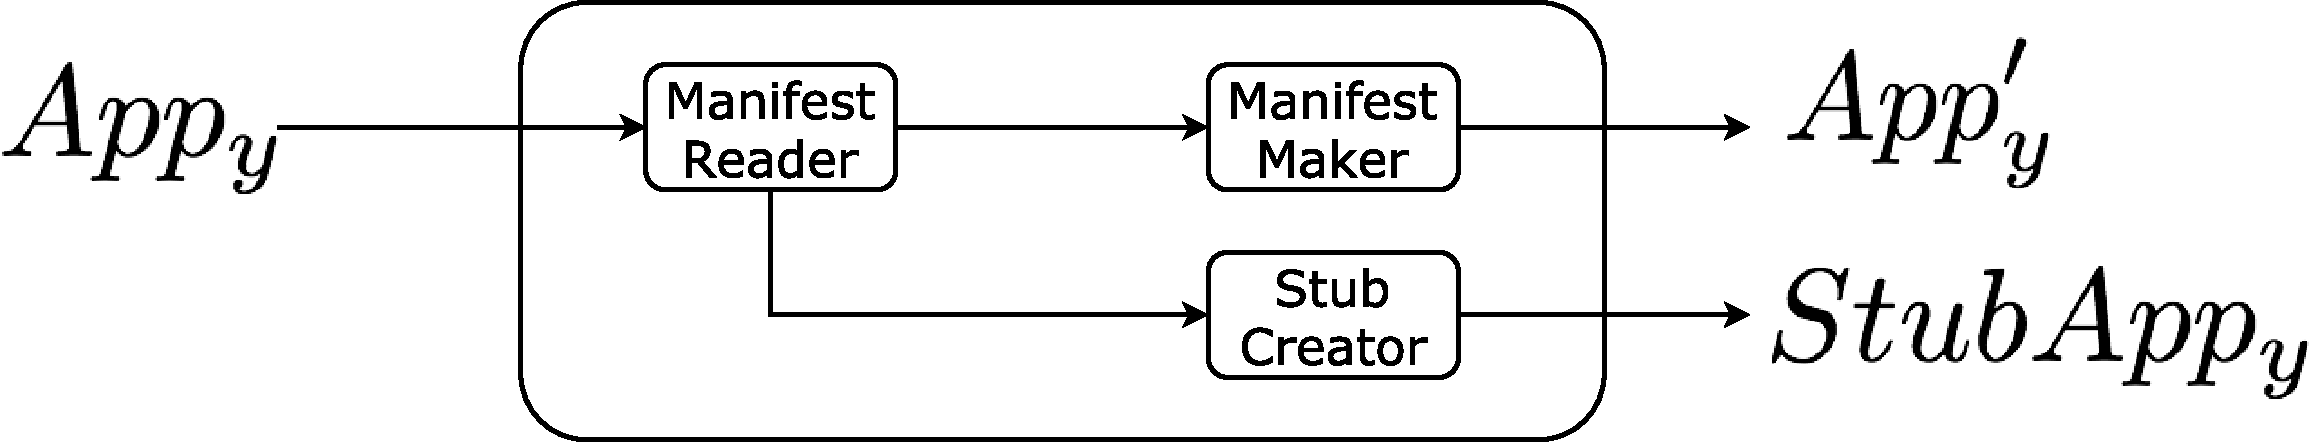
\includegraphics[width=5cm]{stubbo}
				}
			
		\end{tabular}
\end{figure*}
\fi
%--------------------------
\iffalse
\begin{figure*}[!t]
    \centering
    \begin{subfigure}[b]{0.47\textwidth}
        \centering
        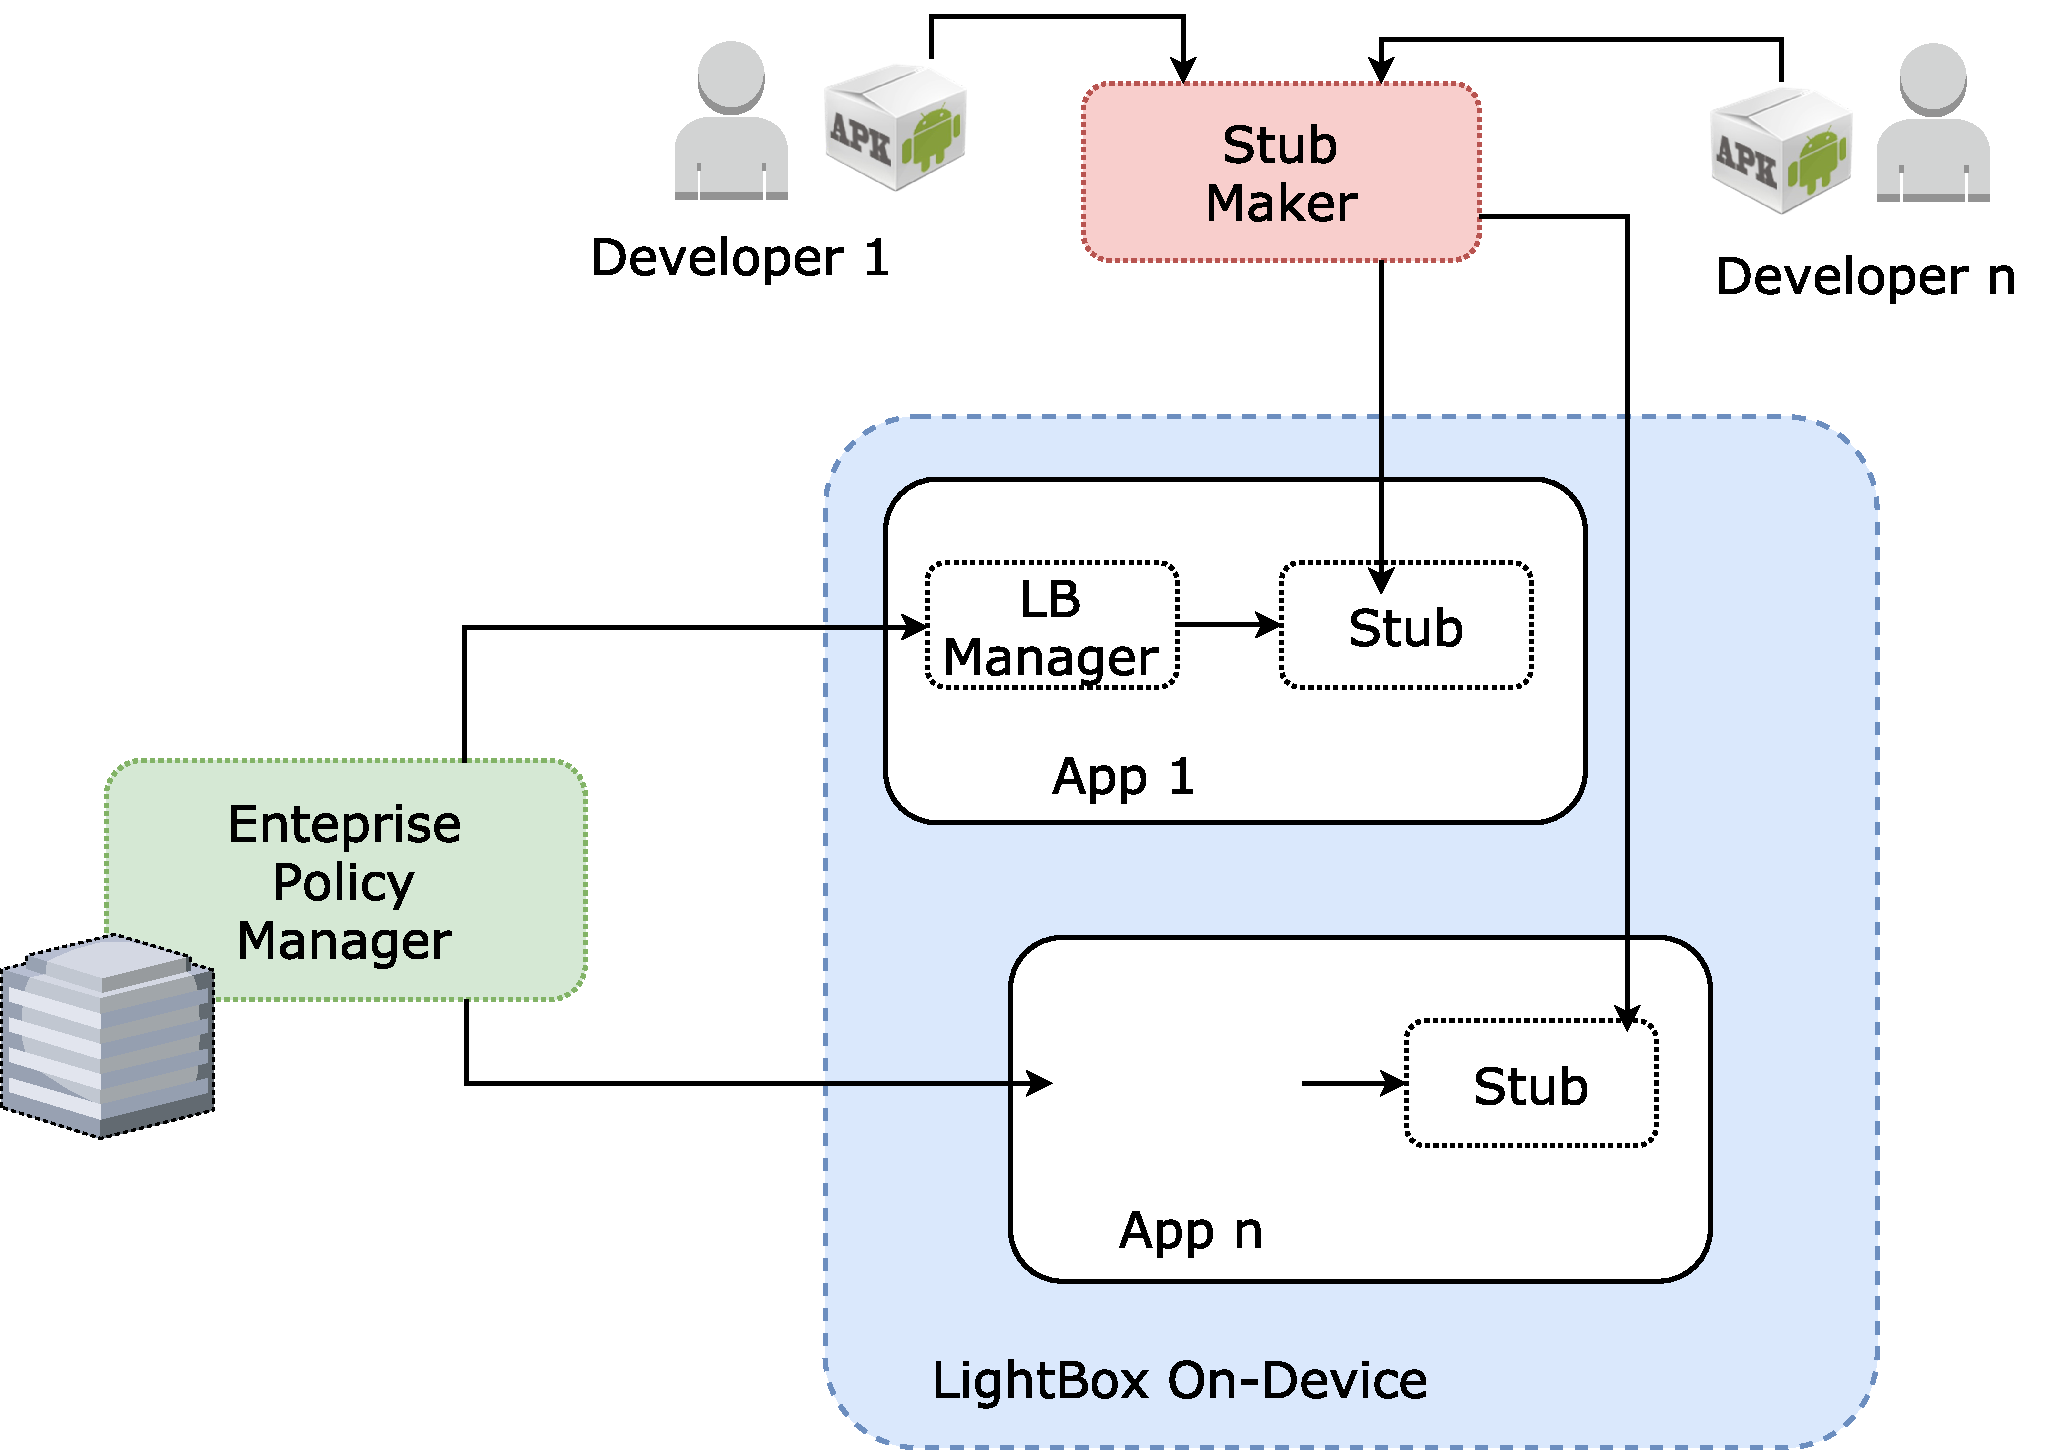
\includegraphics[width=\columnwidth]{design_overview}
        \caption{}
        \label{fig:design_overview}
    \end{subfigure}%
    ~
    \begin{subfigure}[b]{0.29\textwidth}
        \centering
        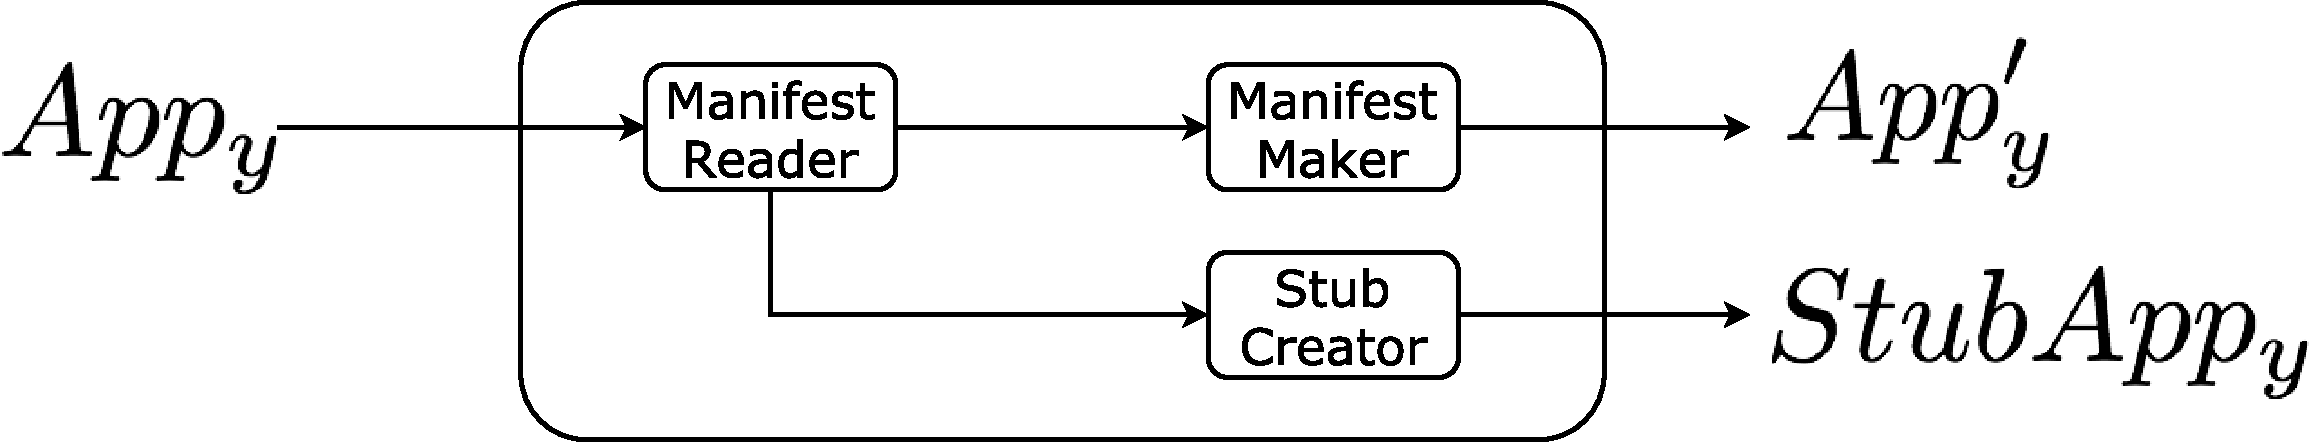
\includegraphics[width=\columnwidth, height=.1\textheight]{stubbo}
        \caption{}
        \label{fig:stubbo}
    \end{subfigure}%
    \caption{a) ... b)....}
\label{fig:example}%
\end{figure*}
\fi
%------------------------------
